%----------------------------------------------------------------------------
\chapter{Writing}\label{app:writing}
%----------------------------------------------------------------------------
\section{Plan before you write: problem to skeleton}\label{app:writing:spine}
Plan the argument before writing prose. Work through the Research and Plan rows of \cref{tab:lifecycle} in order, building on each previous step; after the spine come the figures, the skeleton and the beats.
\begin{description}
  \item[Problem] Start with one paragraph: who has the problem, what goes wrong today, and a concrete scenario showing it. This scenario becomes the running example; the paragraph becomes the first page of \tplref{ch:intro}. Then start the literature review. If you cannot yet write the paragraph, bring your notes to the next consultation and we will write it together.
  \item[Spine] One page fixing the paper's claims, terms and notation. Check every chapter, figure and review against it to catch drift, such as terms, symbols or claims changing between chapters.
  \item[Skeleton mind map] Plan each chapter as paragraph topic sentences with pointers to supporting evidence. Check the argument before expanding those sentences into prose. A mind map on paper or in a tool is a quick way to do this. \Cref{fig:mindmap} shows the expected detail for the guide's fictional paper. \Cref{fig:template-skeleton} shows the template's generic beats in the same form. Use this structure to build a skeleton for your own topic.
  \item[Running example] Choose one scenario to revisit in every chapter. Name it with \texttt{\textbackslash exname} in \texttt{thesis.tex} and introduce it in \tplref{ch:intro}. Use a \texttt{runningexample} box in each chapter to show what its concepts, components, measurements or competitors do with the scenario. The boxes alone should explain the paper.
  \item[Beats] Plan what each paragraph establishes, its evidence, what the example shows and how it leads to the next paragraph. \Cref{app:chapters} gives generic beats for every template heading. Replace them with topic-specific beats at the start of each planned paragraph: \texttt{\textbackslash beat\{establishes\}\{evidence\}\{running example\}\{leads to\}}. These print as todos and disappear from the reviewer PDF.
\end{description}

\begin{figure}[p]
  \centering
  \begin{forest}
    for tree={
      grow'=0, child anchor=west, parent anchor=east, anchor=west,
      font=\scriptsize, edge={gray!60},
      l sep=6mm, s sep=1.2pt, inner sep=1.5pt,
      edge path={\noexpand\path[\forestoption{edge}](!u.parent anchor) -- +(3mm,0) |- (.child anchor)\forestoption{edge label};},
    },
    where level=0{text width=2.4cm, font=\footnotesize}{},
    where level=1{text width=2.5cm}{},
    where level=2{text width=9.3cm}{},
    [{\textbf{Revoking\\credentials\\with bounded\\staleness}}
      [{\textbf{1 Introduction}}
        [{Digital credentials are checked offline, so a revocation must reach the verifier another way \textit{[incident report, cited]}}]
        [{Running example: a revoked diploma that an employer still accepts, because its status copy is stale}]
        [{REQ1 timely revocation (within $\delta$), REQ2 offline checks, REQ3 holder privacy \textit{[Tab. 6.1]}}]
        [{Gap: no existing approach meets REQ1--REQ3 together \textit{[approaches, cited]}}]
        [{C1 model, C2 registry, C3 evaluation; RQ1 correctness, RQ2 scalability, RQ3 robustness \textit{[Fig. 1.1]}}]
      ]
      [{\textbf{2 Background}}
        [{Issuer, holder, verifier; what a revocation status is and how stale a copy can be \textit{[definition, cited]}}]
        [{Accumulators: membership witness, update cost \textit{[definition, cited]}}]
        [{Permissioned ledgers: writers, readers, finality \textit{[definition, cited]}}]
        [{Dolev--Yao adversary and the Tamarin prover \textit{[tool paper, cited]}}]
      ]
      [{\textbf{3 Approach}}
        [{Overview: a check reads one accumulator witness \textit{[Fig. 3.1]}}]
        [{Model: registry state, revocation, staleness of a verifier's copy \textit{[Def. 3.1]}}]
        [{Check: one witness, offline (REQ2), credential not named (REQ3) \textit{[Alg. 3.1]}}]
        [{Adversary: ADV1 a malicious holder replaying an old status proof, ADV2 a Dolev--Yao network adversary \textit{[ADV1--ADV2]}}]
        [{Assumptions: AS1 sound signatures and accumulator, AS2 clock drift at most $\delta$, AS3 honest-but-curious operator \textit{[AS1--AS3]}}]
        [{Out of scope: denial of service, compromised holder devices}]
        [{Lemma 3.1: status proofs are fresh \textit{[Tamarin model; AS1, AS2]}}]
        [{Theorem 3.1 = SG1: under AS1--AS3, against ADV1 and ADV2, a verifier rejects every credential revoked more than $\delta$ before the check \textit{[Tamarin proof]}}]
        [{Example: the diploma presented with an old status proof is rejected}]
      ]
      [{\textbf{4 Implementation}}
        [{Architecture: registry service, verifier library, reused ledger \textit{[Fig. 3.1]}}]
        [{Design: signed accumulator values, not ledger reads \textit{[alternative rejected]}}]
        [{The verifier's check: signed and younger than $\delta$ \textit{[listing, tests]}}]
        [{Code and scripts archived on Zenodo, with the rerun command \textit{[archived code]}}]
      ]
      [{\textbf{5 Evaluation}}
        [{Setup: one 8-core cloud VM, 10 runs, fresh issuer sets \textit{[rerun command]}}]
        [{RQ1 correctness: proofs per guarantee, tests per requirement \textit{[Tab. 5.1]}}]
        [{The scenario before and after, as a sequence chart \textit{[Fig. 5.1]}}]
        [{RQ2 scalability: checks stay within one round trip up to 10\,000 issuers; a list-based baseline grows linearly \textit{[Fig. 5.2]}}]
        [{Storage grows with the credentials ever issued \textit{[Fig. 5.2]}}]
        [{RQ3 robustness: a ledger node crash, a revocation burst, clock drift and $\delta$ varied \textit{[Tab. 5.2, Fig. 5.3]}}]
        [{Threats to validity: synthetic issuer sets, one cloud VM}]
      ]
      [{\textbf{6 Related work}}
        [{Family A: how it works, which of REQ1--REQ3 it gives up \textit{[approaches, cited]}}]
        [{Family B: how it works, which of REQ1--REQ3 it gives up \textit{[approaches, cited]}}]
        [{Family C: how it works, which of REQ1--REQ3 it gives up \textit{[approaches, cited]}}]
        [{Gap matrix: no family meets REQ1--REQ3 together \textit{[Tab. 6.1, Fig. 6.1]}}]
      ]
      [{\textbf{7 Conclusion}}
        [{C1--C3 restated with their evidence \textit{[Thm 3.1, Fig. 5.2, Tab. 5.1]}}]
        [{LIM1 synthetic workloads \textit{[threats to validity]}}]
        [{LIM2 the registry cannot force an issuer to revoke \textit{[scope of SG1]}}]
        [{Future work: real issuer workloads; holding issuers to their revocation duty}]
      ]
    ]
  \end{forest}
  \caption{A skeleton for the fictional credential revocation paper developed in \cref{app:chapters}. Each leaf is a paragraph's topic sentence; bracketed italics identify its evidence, such as a theorem, model, table, figure or citation.}\label{fig:mindmap}
\end{figure}


\begin{figure}[p]
  \centering
  \begin{forest}
    for tree={
      grow'=0, child anchor=west, parent anchor=east, anchor=west,
      font=\scriptsize, edge={gray!60},
      l sep=6mm, s sep=1.2pt, inner sep=1.5pt,
      edge path={\noexpand\path[\forestoption{edge}](!u.parent anchor) -- +(3mm,0) |- (.child anchor)\forestoption{edge label};},
    },
    where level=0{text width=2.4cm, font=\footnotesize}{},
    where level=1{text width=2.5cm}{},
    where level=2{text width=9.3cm}{},
    [{\textbf{The template's beats}}
      [{\textbf{1 Introduction}}
        [{Context: why the field matters now \textit{[a trend, a regulation or an incident, cited]}}]
        [{Problem: the concrete problem, ending in a one-sentence statement \textit{[the running example]}}]
        [{Requirements: what a solution must do \textit{[one requirement per failure of the example; the rows of the gap matrix]}}]
        [{Gap: no existing approach meets them together \textit{[the closest approaches, cited]}}]
        [{Contributions: what this work claims, as checkable items \textit{[the chapters behind each]}}]
      ]
      [{\textbf{2 Background}}
        [{The first concept the approach relies on; notation defined once \textit{[a definition and a citation]}}]
        [{The second concept \textit{[a definition and a citation]}}]
      ]
      [{\textbf{3 Approach}}
        [{Overview: how it works end to end \textit{[the architecture figure]}}]
        [{The formal model or the design decisions \textit{[each decision with the alternative rejected]}}]
        [{Threat model: the adversary's capabilities, who is trusted, the cryptographic assumptions, what is out of scope, and the guarantees \textit{[a proof, a mechanised proof or a measurement per guarantee]}}]
      ]
      [{\textbf{4 Implementation}}
        [{What was built and how it realises the approach \textit{[components mapped to code; the archived artifact]}}]
        [{Design decisions and the problems a straightforward build runs into \textit{[each with the alternative rejected]}}]
        [{The part that did not exist before \textit{[the key listing and the tests that cover it]}}]
      ]
      [{\textbf{5 Evaluation}}
        [{Setup: how the measurements were made \textit{[hardware, versions, workloads, repetitions, the rerun command]}}]
        [{Correctness on the example and on every requirement case \textit{[test, proof or model-checking results]}}]
        [{How the cost grows with the input \textit{[the scalability figure]}}]
        [{Behaviour when the assumptions are stressed \textit{[the robustness table, with each perturbation's setup]}}]
        [{Threats to validity and what was done about each \textit{[the mitigations]}}]
      ]
      [{\textbf{6 Related work}}
        [{How each family of approaches works and where it falls short \textit{[citations, the positioning figure and the gap matrix]}}]
        [{The gap in one sentence, closed by this work \textit{[the gap matrix and the evaluation results]}}]
      ]
      [{\textbf{7 Conclusion}}
        [{Each contribution and its evidence \textit{[the chapters behind C1--C3]}}]
        [{What is still open, and the next step for each limitation \textit{[the threats to validity]}}]
      ]
    ]
  \end{forest}
  \caption{The template's generic beats from \cref{app:chapters}: one leaf per beat, with its topic followed by evidence in brackets. Develop these for your topic, as in \cref{fig:mindmap}. Add more leaves where the contribution needs them and fewer elsewhere.}\label{fig:template-skeleton}
\end{figure}

\section{The essentials}\label{app:writing:essentials}
The list below defines the two dozen elements expected in every paper of this kind, including the problem, requirements, leading figure, threat model, research questions, gap matrix and summary with evidence. These are the named items in \cref{fig:template-skeleton} that reviewers look for. Each row gives the review-sheet criterion that scores it.

The lint calls these items the \emph{essentials}. Their status appears on the draft PDF's Checks page and at the start of the CI job summary. The list is defined in \texttt{scripts/lint/essentials.lua}; \texttt{make essentials} generates this section from it. The requirements still apply if you delete the skeleton chapters. Each row links to a worked example in \cref{app:chapters}.

% generated by texlua scripts/lint.lua essentials --guide (make essentials); do not edit
\definecolor{lintaccent}{RGB}{155,28,28}\definecolor{lintmute}{gray}{0.38}
\providecommand{\lintdisc}[3]{\tikz[baseline=-.6ex]{\draw[#2,line width=.45pt,fill=white] (0,0) circle (#1);\ifcase#3\relax\or\fill[#2] (0,0) -- (0,#1) arc[start angle=90,end angle=0,radius=#1] -- cycle;\or\fill[#2] (0,0) -- (0,#1) arc[start angle=90,end angle=-90,radius=#1] -- cycle;\or\fill[#2] (0,0) -- (0,#1) arc[start angle=90,end angle=-180,radius=#1] -- cycle;\or\fill[#2] (0,0) circle (#1);\fi}}
\providecommand{\lintball}[2][black]{\lintdisc{.62ex}{#1}{#2}}
\providecommand{\lintbigball}[2][black]{\lintdisc{.8ex}{#1}{#2}}
The lint places each essential on a ladder of five levels: \lintball{0} missing; \lintball{1} a placeholder, only TODO or the template's own text; \lintball{2} started, your own text but not enough of it; \lintball{3} written; \lintball{4} used where the argument needs it. An essential with no condition for its use is \lintball{4} once written. The phase in \texttt{thesis.tex} asks every essential for a level: \textsc{plan} \lintball{1}, \textsc{draft} \lintball{2}, \textsc{polish} and \textsc{final} \lintball{4}. An essential is found by its label first, then by a heading that contains one of the words given. Text is your own when it is neither a TODO line nor a line of the template, and floats, tagged lists and example boxes count toward their own essentials, not toward the text around them.

{\small\begin{xltabular}{\linewidth}{@{}>{\raggedright\arraybackslash}p{.25\linewidth}>{\raggedright\arraybackslash}X>{\raggedright\arraybackslash}p{.3\linewidth}@{}}
\toprule \textbf{Essential} & \textbf{What it is, and why} & \textbf{Written, and used} \\ \midrule \endfirsthead
\toprule \textbf{Essential} & \textbf{What it is, and why} & \textbf{Written, and used} \\ \midrule \endhead \bottomrule \endlastfoot
\multicolumn{3}{@{}l}{\textsc{Front matter}} \\
\textbf{Abstract and Kivonat}\newline{\footnotesize\color{lintmute}\texttt{\textbackslash chapter*\{Kivonat\}} and \texttt{\{Abstract\}}}\newline{\footnotesize In action: \cref{app:writing:abstract}} & The paper in one paragraph, in English and in Hungarian; the reviewer reads it first and the registration carries it.\hfill{\footnotesize\color{lintmute}(E)} & 100 own words in each.\newline Written is enough. \\
\addlinespace[.8ex]\multicolumn{3}{@{}l}{\textsc{Introduction}} \\
\textbf{Context}\newline{\footnotesize\color{lintmute}\texttt{par:context}, or a heading with \emph{context} or \emph{motivation}}\newline{\footnotesize In action: \cref{app:chapters:context}} & Why the topic matters now: a trend, a regulation or an incident, cited; relevance is scored in C.\hfill{\footnotesize\color{lintmute}(C, E)} & 40 own words.\newline Written is enough. \\
\textbf{Problem statement}\newline{\footnotesize\color{lintmute}\texttt{par:problem}, or a heading with \emph{problem}}\newline{\footnotesize In action: \cref{app:chapters:problem}} & The concrete problem, ending in a one-sentence statement; the sheet's E names the problem statement as a must.\hfill{\footnotesize\color{lintmute}(E)} & 40 own words.\newline Written is enough. \\
\textbf{Running example}\newline{\footnotesize\color{lintmute}\texttt{\textbackslash exname} and the example box}\newline{\footnotesize In action: \cref{app:chapters:problem}} & One small scenario, named once in thesis.tex (\textbackslash{}exname) and revisited in a box in every chapter, so the reader can follow each step.\hfill{\footnotesize\color{lintmute}(A)} & Named, and the introduction's box in your own words.\newline Used when an example box in every main chapter. \\
\textbf{Requirements}\newline{\footnotesize\color{lintmute}items labelled \texttt{req:}}\newline{\footnotesize In action: \cref{app:chapters:requirements}} & What a solution must do, one checkable item each; they are the rows of the gap matrix and the yardstick of the evaluation.\hfill{\footnotesize\color{lintmute}(D/1)} & Every item in your own words.\newline Used when each requirement is referenced in the related work and in the evaluation, and each derived requirement (dr:) in the evaluation. \\
\textbf{Gap, in brief}\newline{\footnotesize\color{lintmute}\texttt{par:gap}, or a heading with \emph{gap}}\newline{\footnotesize In action: \cref{app:chapters:introgap}} & That no existing approach meets the requirements together; the novelty claim, made before the full comparison.\hfill{\footnotesize\color{lintmute}(D/1)} & 40 own words.\newline Used when it points to the full comparison: the related-work chapter, the gap matrix or the positioning figure. \\
\textbf{Leading figure}\newline{\footnotesize\color{lintmute}\texttt{fig:overview}}\newline{\footnotesize In action: \cref{fig:guide:overview}} & The problem, the contributions and the headline result in one picture; the reviewer looks here first.\hfill{\footnotesize\color{lintmute}(B/1)} & Your own content, and a caption of at least a sentence.\newline Used when it is referenced from the text. \\
\textbf{Contributions}\newline{\footnotesize\color{lintmute}items labelled \texttt{c:}}\newline{\footnotesize In action: \cref{app:chapters:contributions}} & What this work claims, as checkable items; the sheet's E names stating the main contribution as a must.\hfill{\footnotesize\color{lintmute}(E)} & Every item in your own words.\newline Used when each contribution points to the chapter that delivers it and is referenced in the conclusion. \\
\addlinespace[.8ex]\multicolumn{3}{@{}l}{\textsc{Approach}} \\
\textbf{Architecture figure}\newline{\footnotesize\color{lintmute}\texttt{fig:architecture}}\newline{\footnotesize In action: \cref{fig:guide:architecture}} & The approach end to end, with what is yours set apart from what is reused.\hfill{\footnotesize\color{lintmute}(B/1)} & Your own content, and a caption of at least a sentence.\newline Used when it is referenced from the text. \\
\textbf{Threats}\newline{\footnotesize\color{lintmute}items labelled \texttt{thr:}}\newline{\footnotesize In action: \cref{app:chapters:adversary}} & Who the adversary is and what it can do; a reviewer of a security topic looks for it first.\hfill{\footnotesize\color{lintmute}(D/2)} & Every item in your own words.\newline Used when each threat is referenced in the approach, where a guarantee or an assumption meets it. \\
\textbf{Assumptions}\newline{\footnotesize\color{lintmute}items labelled \texttt{asm:}}\newline{\footnotesize In action: \cref{app:chapters:assumptions}} & Who is trusted and which properties the guarantees rest on, stated so a reviewer can check them.\hfill{\footnotesize\color{lintmute}(D/2)} & Every item in your own words.\newline Used when each assumption is referenced in the approach, by a guarantee or a proof. \\
\textbf{Guarantees}\newline{\footnotesize\color{lintmute}items labelled \texttt{g:}}\newline{\footnotesize In action: \cref{app:chapters:guarantees}} & What the approach guarantees under the assumptions, against the threats; each is what the evaluation checks.\hfill{\footnotesize\color{lintmute}(D/2)} & Every item in your own words.\newline Used when each guarantee is referenced in the evaluation, as a row of the correctness table. \\
\addlinespace[.8ex]\multicolumn{3}{@{}l}{\textsc{Evaluation}} \\
\textbf{Research questions}\newline{\footnotesize\color{lintmute}items labelled \texttt{rq:}}\newline{\footnotesize In action: \cref{app:chapters:research-questions}} & The questions the evaluation answers: correctness, scale and robustness at least.\hfill{\footnotesize\color{lintmute}(E)} & Every item in your own words.\newline Used when each research question is referenced in the evaluation, where it is answered. \\
\textbf{Setup and artifact}\newline{\footnotesize\color{lintmute}\texttt{sec:setup}, or a heading with \emph{setup}}\newline{\footnotesize In action: \cref{app:chapters:setup}} & How the measurements were made, so each can be checked, and where the archived artifact is.\hfill{\footnotesize\color{lintmute}(D/2)} & 100 own words.\newline Used when the evaluation cites the archived artifact with a real DOI. \\
\textbf{Correctness}\newline{\footnotesize\color{lintmute}\texttt{tab:correctness}}\newline{\footnotesize In action: \cref{tab:guide:correctness}} & How each guarantee and requirement was checked: proved, tested or model-checked, with the result.\hfill{\footnotesize\color{lintmute}(D/2)} & Your own content, and a caption of at least a sentence.\newline Used when it is referenced from the text, and every guarantee (g:) has a row in it. \\
\textbf{Scalability}\newline{\footnotesize\color{lintmute}\texttt{sec:scalability}, or a heading with \emph{scalab} or \emph{scaling} or \emph{performance}}\newline{\footnotesize In action: \cref{app:chapters:scalability}} & How the cost grows with the input; the review sheet scores the evaluation's depth in E.\hfill{\footnotesize\color{lintmute}(E)} & 100 own words.\newline Used when the section holds a figure or table that the text references. \\
\textbf{Robustness}\newline{\footnotesize\color{lintmute}\texttt{sec:robustness}, or a heading with \emph{robust}}\newline{\footnotesize In action: \cref{app:chapters:robustness}} & How the system behaves when its assumptions are stressed; scored apart from scalability.\hfill{\footnotesize\color{lintmute}(E)} & 100 own words.\newline Used when the section holds a figure or table that the text references. \\
\textbf{Threats to validity}\newline{\footnotesize\color{lintmute}\texttt{sec:validity}, or a heading with \emph{validity}}\newline{\footnotesize In action: \cref{app:chapters:validity}} & What could make the results wrong or not generalise, and what was done about each.\hfill{\footnotesize\color{lintmute}(D/2)} & 100 own words.\newline Written is enough. \\
\addlinespace[.8ex]\multicolumn{3}{@{}l}{\textsc{Related work}} \\
\textbf{Positioning figure}\newline{\footnotesize\color{lintmute}\texttt{fig:positioning}}\newline{\footnotesize In action: \cref{fig:guide:positioning}} & The related work on the two properties that separate it most, with this work in the cell no one else reaches.\hfill{\footnotesize\color{lintmute}(B/2)} & Your own content, and a caption of at least a sentence.\newline Used when it is referenced from the text. \\
\textbf{Gap matrix}\newline{\footnotesize\color{lintmute}\texttt{tab:related}}\newline{\footnotesize In action: \cref{tab:guide:related}} & Each requirement against the closest approaches: every other approach misses something, this work meets all.\hfill{\footnotesize\color{lintmute}(D/1)} & Your own content, and a caption of at least a sentence.\newline Used when rows are the requirements, this work's column is all met with pointers to results, and every other approach misses one. \\
\textbf{The gap}\newline{\footnotesize\color{lintmute}\texttt{sec:gap}, or a heading with \emph{gap}}\newline{\footnotesize In action: \cref{app:chapters:gap}} & The gap in one sentence, shown closed by this work's results.\hfill{\footnotesize\color{lintmute}(D/1)} & 100 own words.\newline Used when it is based on the gap matrix (references tab:related). \\
\addlinespace[.8ex]\multicolumn{3}{@{}l}{\textsc{Conclusion}} \\
\textbf{Summary with evidence}\newline{\footnotesize\color{lintmute}\texttt{sec:summary}, or a heading with \emph{summary}}\newline{\footnotesize In action: \cref{app:chapters:summary}} & Each contribution restated with the result behind it; the reviewer checks here that the promises were kept.\hfill{\footnotesize\color{lintmute}(E)} & 100 own words.\newline Used when it cites an evaluation result: the evaluation chapter, a research question, a figure, a table or a theorem. \\
\textbf{Limitations}\newline{\footnotesize\color{lintmute}items labelled \texttt{lim:}}\newline{\footnotesize In action: \cref{app:chapters:future}} & What this work does not do, stated before a reviewer finds it.\hfill{\footnotesize\color{lintmute}(E)} & Every item in your own words.\newline Written is enough. \\
\textbf{Future work}\newline{\footnotesize\color{lintmute}\texttt{sec:future}, or a heading with \emph{future}}\newline{\footnotesize In action: \cref{app:chapters:future}} & What is still open, and the next step that would lift each limitation.\hfill{\footnotesize\color{lintmute}(E)} & 100 own words.\newline Written is enough. \\
\end{xltabular}}


\section{The leading figure (vezérábra)}\label{app:writing:figure}
The leading figure (\tplref{fig:overview}) shows the problem, your contributions and the result in one picture. Decide what the reader should learn, then draw it and write a caption that makes it understandable on its own. Use the \texttt{ours} TikZ style to colour all your components blue. The problem is red, the result green, and reused or external parts grey (\texttt{prior}). Every work has at least two components; give all of yours the same blue and explain the colours in the caption. If ownership is unclear, a reviewer may attribute only the smallest part to you.

Draft the figure during research and keep exploring it until the spine is agreed. Drawing often helps clarify the argument. \Cref{fig:collage} shows four examples from our group.

\begin{figure}[!ht]
  \centering
  \begin{subfigure}[t]{0.48\linewidth}
    \centering
    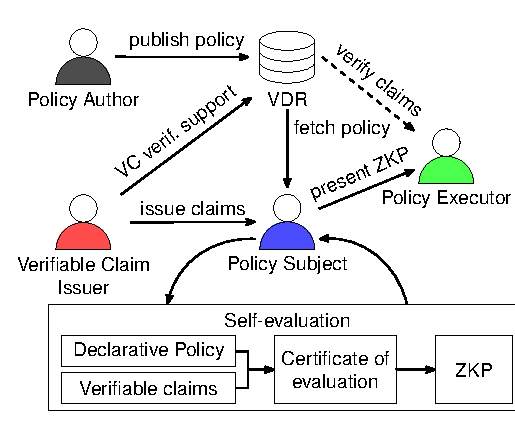
\includegraphics[width=\linewidth,height=5.2cm,keepaspectratio]{guide/figures/collage/eurocybersec2024}
    \caption{A subject evaluates its own policy and proves the result in zero knowledge. The figure shows actors and flows.}\label{fig:collage:ecs}
  \end{subfigure}\hfill
  \begin{subfigure}[t]{0.48\linewidth}
    \centering
    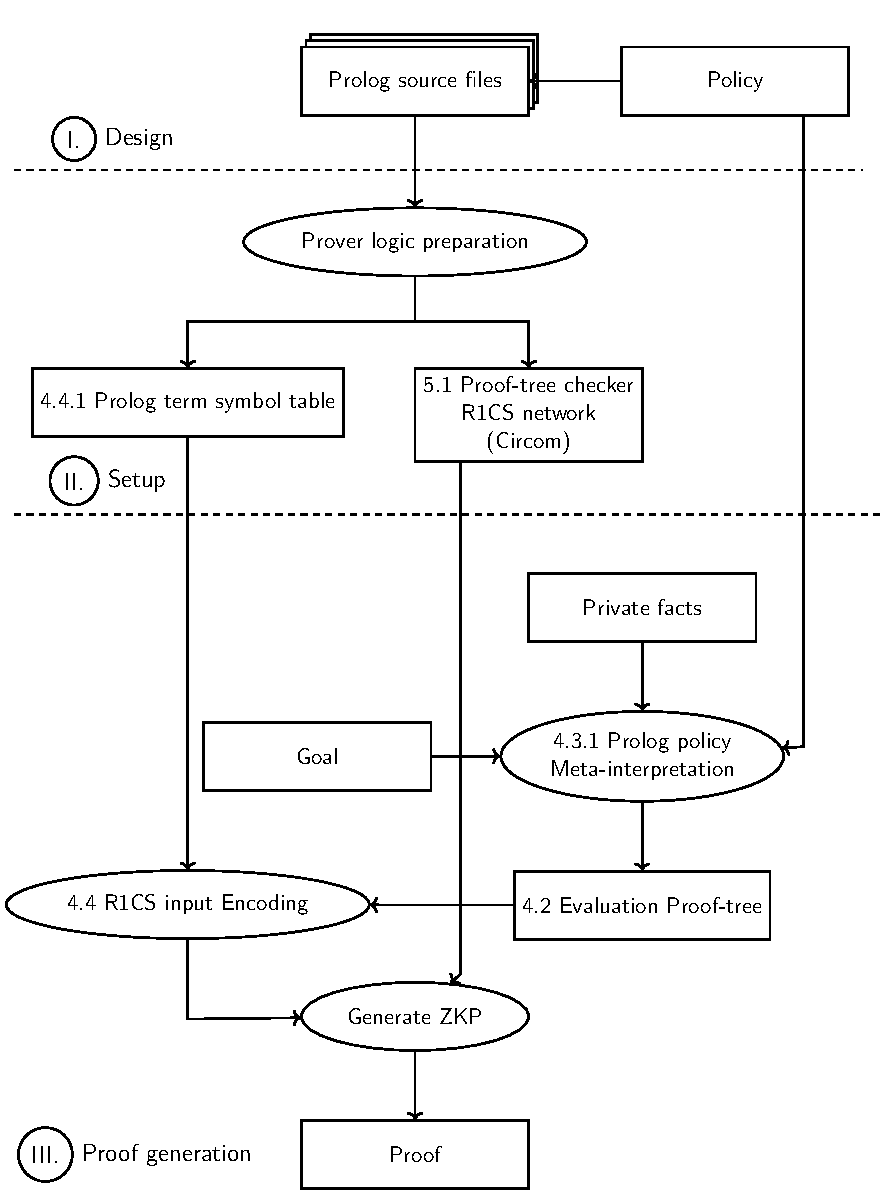
\includegraphics[width=\linewidth,height=5.2cm,keepaspectratio]{guide/figures/collage/tdk2023}
    \caption{The same idea in a TDK paper. The toolchain shows each stage from policy to proof and locates the contribution.}\label{fig:collage:tdk}
  \end{subfigure}

  \medskip
  \begin{subfigure}[t]{0.48\linewidth}
    \centering
    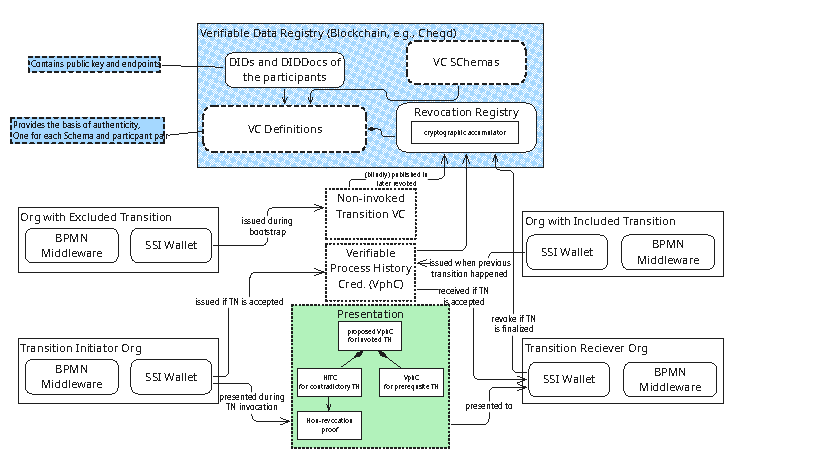
\includegraphics[width=\linewidth,height=5.2cm,keepaspectratio]{guide/figures/collage/bpm2025}
    \caption{Self-orchestrated business collaborations, with architecture and data model in one figure.}\label{fig:collage:bpm25}
  \end{subfigure}\hfill
  \begin{subfigure}[t]{0.48\linewidth}
    \centering
    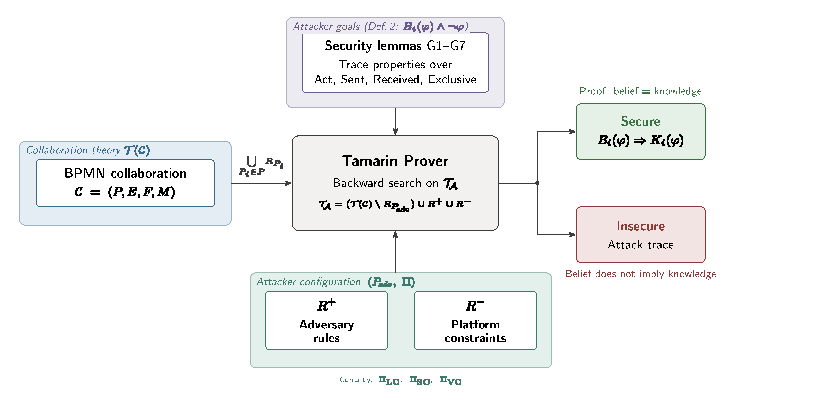
\includegraphics[width=\linewidth,height=5.2cm,keepaspectratio]{guide/figures/collage/bpm2026}
    \caption{From a BPMN collaboration to a security analysis: inputs on the left, the method in the middle, the verdicts on the right.}\label{fig:collage:bpm26}
  \end{subfigure}
  \caption{Leading figures drawn before their papers: (a) self-evaluated policies at EuroCyberSec 2024~\cite{guide:farkas2024selfevaluated}, (b) the 2023 TDK paper behind it~\cite{guide:farkas2023tdk}, (c) self-orchestrated business collaborations~\cite{guide:farkas2025selforchestration}, and (d) formal security analysis of BPMN collaborations~\cite{guide:farkas2026trustnopool}.}\label{fig:collage}
\end{figure}

When the contribution is spread over several chapters, \cref{app:writing:depgraph} draws the whole paper instead.

\section{An alternative: the paper as a dependency graph}\label{app:writing:depgraph}
The skeleton mind map (\cref{fig:mindmap}) is a tree of chapters and their paragraphs. Draw an arrow from each paragraph to every paragraph that needs it, and the tree becomes a dependency graph of the paper (\cref{fig:depgraph}). Lay it out in bands, one per chapter in reading order, with each band's paragraphs in their order in the chapter. Colour green the paragraphs that deliver a contribution, tag each with its contribution, and leave the rest white. The green is for the reviewer: before reading a sentence, they see where your contribution is, how much of the paper it fills, what it stands on, and which evaluation question tests it. Green marks paragraphs here, not components, so the architecture figure keeps the blue of \texttt{ours} for the parts of the system you built.

\begin{figure}[!ht]
  \centering
  \begin{tikzpicture}[
      x=25mm, y=-17mm,
      para/.style={draw=gray!60, fill=white, rounded corners=1pt, text width=20mm, minimum height=10mm,
        align=center, font=\footnotesize, inner sep=2pt, execute at begin node={\hyphenpenalty=10000}},
      contrib/.style={para, draw=green!50!black, line width=1.1pt, fill=green!15},
      dep/.style={-Stealth, gray!70, semithick}]
    % One band per chapter, in reading order; within a band, paragraphs keep their order in the chapter.
    \begin{scope}[on background layer]
      \foreach \r/\chap in {0/Introduction, 1/Background, 2/Approach, 3/Implementation,
                            4/Evaluation, 5/Related work, 6/Conclusion} {
        \pgfmathsetmacro{\n}{int(\r+1)}
        \pgfmathparse{mod(\r,2) ? "white" : "gray!8"}
        \fill[\pgfmathresult] (-1.6,\r-0.47) rectangle (5.5,\r+0.47);
        \node[anchor=west, font=\footnotesize] at (-1.58,\r) {\textbf{\n}~\chap};
      }
    \end{scope}
    \node[para]    (problem)  at (0,0) {Problem: a stale status};
    \node[para]    (req)      at (1,0) {REQ1--REQ3};
    \node[para]    (gap)      at (2,0) {Gap: none meets all three};
    \node[para]    (claims)   at (3,0) {Contributions C1--C3};
    \node[para]    (cred)     at (0,1) {Revocation status};
    \node[para]    (acc)      at (1,1) {Accumulators};
    \node[para]    (ledger)   at (2,1) {Permissioned ledgers};
    \node[para]    (dy)       at (3,1) {Dolev--Yao and Tamarin};
    \node[contrib] (model)    at (0,2) {\textbf{C1} Registry model};
    \node[contrib] (check)    at (1,2) {\textbf{C1} Check with one witness};
    \node[para]    (threat)   at (3,2) {Adversary and assumptions};
    \node[contrib] (thm)      at (4,2) {\textbf{C1} Theorem: SG1};
    \node[contrib] (arch)     at (0,3) {\textbf{C2} Architecture};
    \node[contrib] (design)   at (1,3) {\textbf{C2} Signed values};
    \node[contrib] (code)     at (2,3) {\textbf{C2} The check, tested};
    \node[contrib] (rq1)      at (2,4) {\textbf{C3} RQ1 correctness};
    \node[contrib] (rq2)      at (3,4) {\textbf{C3} RQ2 scalability};
    \node[contrib] (rq3)      at (4,4) {\textbf{C3} RQ3 robustness};
    \node[para]    (validity) at (5,4) {Threats to validity};
    \node[para]    (families) at (0,5) {Families A--C};
    \node[para]    (matrix)   at (1,5) {Gap matrix};
    \node[para]    (summary)  at (3,6) {Summary of C1--C3};
    \node[para]    (limits)   at (4,6) {Limitations};
    \node[para]    (future)   at (5,6) {Future work};
    % An arrow points from a paragraph to the paragraph that needs it.
    \draw[dep] (problem) -- (req);
    \draw[dep] (req) -- (gap);
    \draw[dep] (gap) -- (claims);
    \draw[dep] (cred) -- (model);
    \draw[dep] (acc) -- (check);
    \draw[dep] (model) -- (check);
    \draw[dep] (dy) -- (threat);
    \draw[dep] (threat) -- (thm);
    \draw[dep] (check.south east) .. controls (2.1,2.62) and (3.3,2.62) .. (thm.south west);
    \draw[dep] (check) -- (arch);
    \draw[dep] (ledger) -- (design.north east);
    \draw[dep] (arch) -- (design);
    \draw[dep] (design) -- (code);
    \draw[dep] (thm.250) -- (rq1.north east);
    \draw[dep] (code) -- (rq1);
    \draw[dep] (code.east) -| ($(rq2.north)+(-0.2,0)$);
    \draw[dep] (thm) -- (rq3);
    \draw[dep] (families) -- (matrix);
    \draw[dep] (rq1) -- (summary);
    \draw[dep] (rq2) -- (summary);
    \draw[dep] (rq3) -- (summary);
    \draw[dep] (validity) -- (limits);
    \draw[dep] (limits) -- (future);
  \end{tikzpicture}
  \caption{The guide's running example as a dependency graph: each contribution stands on the background and leads to an evaluation question. One band per chapter in reading order, one box per paragraph in its order within the chapter, and an arrow from a paragraph to each paragraph that needs it. Green boxes deliver the contribution in their tag, white boxes are context, and every arrow runs to a later chapter or rightwards within one. It is the paper of \cref{fig:mindmap} with fewer boxes: the figure keeps the paragraphs that carry the argument, not all of them.}\label{fig:depgraph}
\end{figure}

It can take either of two places in the paper. As \tplref{fig:overview}, it suits a work whose contribution is a model, a tool and an evaluation spread over several chapters, which a problem-to-result picture would flatten into one box; the green has to read at a glance, so merge a chapter's paragraphs into its sections when there are many. As the figure of the structure paragraph at the end of the introduction (\cref{app:chapters:structure}), it replaces the list of chapters: the paragraph says what the bands, arrows and colours mean, and the figure shows the rest.

Drawing it also checks the skeleton before any prose exists. Every arrow should run down to a later chapter or right within one; an arrow pointing up or left is a paragraph that needs something the reader has not reached yet, so move one of the two, or say where the missing part comes. A green box with no path to an evaluation question is a contribution the paper claims but does not back. A background box that no arrow leaves is background the paper does not use. Draw only the arrows a reader needs to follow the argument: the figure shows where the contribution is, not every cross-reference.

\section{Figures}\label{app:writing:figures}
We recommend TikZ for every figure: drawn in the paper repository, it matches the paper's fonts, scales cleanly and allows late edits; \cref{app:latex} covers the template's TikZ and pgfplots setup. Sketch in \href{https://www.drawio.com/}{draw.io} while exploring, then redraw in TikZ after agreeing the spine. You can also export draw.io and Inkscape drawings as SVG and include them with \texttt{\textbackslash includesvg} (\cref{app:latex:figures}), so the text stays sharp. Raster images and screenshots, for example a figure from another paper, are allowed only with a reason, and they are not vector figures. Use any other exported PDF only as a last resort. Generate plots with pgfplots from the CSV written by \texttt{just reproduce}, so measurements update the figures automatically. Label every axis with its unit.

The target for figure text is 10\,pt in print, as the call says: \enquote{10 pt alatti betűméret kerülendő címkéken is} (\cref{app:tdk:form}). Where 10\,pt does not fit, we accept 8\,pt as the floor. The lint flags only text below 8\,pt, so text between 8 and 10\,pt is yours to check.

\section{Captions}\label{app:writing:captions}
Figures and captions alone should let a reader follow the paper. Start each caption with the claim the figure supports. Then give the context needed to understand it: the question answered, the concept measured, assumptions in the setup, or why a curve bends. Avoid repeating information already clear from the axes and legend. Use two or three sentences for a diagram and as many as needed to explain a result. For examples, read the Nature captions in \citet{guide:gulyas2015navigable}; \cref{fig:caption-example} applies this style in the template.

\begin{figure}[!ht]
  \centering
  \begin{tikzpicture}
    \begin{groupplot}[group style={group size=2 by 1, horizontal sep=1.6cm}, width=0.5\linewidth, height=5cm,
      xmode=log, log basis x=10, xlabel={Issuers in the registry}, grid=major, tick label style={font=\footnotesize}, label style={font=\footnotesize}, legend style={font=\footnotesize, at={(0.03,0.97)}, anchor=north west}]
      \nextgroupplot[ylabel={Median check latency [ms]}, ymode=log, title={(a)}, title style={font=\footnotesize}]
        \addplot+[mark=*, blue!70!black] coordinates {(10,31) (100,33) (1000,35) (10000,38)};
        \addplot+[mark=square*, gray] coordinates {(10,34) (100,61) (1000,310) (10000,2900)};
        \addplot[dashed, red!70!black] coordinates {(10,40) (10000,40)};
        \legend{this work, list-based baseline, one round trip}
      \nextgroupplot[ylabel={Registry size [MB]}, title={(b)}, title style={font=\footnotesize}, ymode=log]
        \addplot+[mark=*, blue!70!black] coordinates {(10,2) (100,12) (1000,110) (10000,1050)};
        \addplot+[mark=square*, gray] coordinates {(10,1) (100,3) (1000,21) (10000,190)};
    \end{groupplot}
  \end{tikzpicture}
  \caption{\textbf{Revocation checks stay within one network round trip up to 10\,000 issuers, while the list-based baseline grows linearly.} This answers RQ2: can a national-scale registry check a credential without noticeable delay? Each check reads one accumulator witness regardless of issuer count; the baseline scans the issuer's list. Storage in panel (b) grows with all credentials ever issued, but the robustness analysis shows it fits on a single server. Medians of 10 runs with fresh issuer sets on one 8-core BME cloud VM. (Illustrative numbers for the guide's running example.)}\label{fig:caption-example}
\end{figure}

\section{The abstract}\label{app:writing:abstract}
We require the abstract to explain why the work is worth reading. We read it at registration, then the committee uses it to assign reviewers, who read it first too. Show that the topic is \textbf{relevant}, solving it is \textbf{non-trivial}, the contribution is \textbf{novel} and the result is \textbf{correct}: these are the four things the whole paper argues (\cref{app:chapters}). Follow \weblink{https://www.nature.com/documents/nature-summary-paragraph.pdf}{Nature's summary paragraph guide}. The template abstract has placeholders for its seven steps.

The faculty asks for Hungarian and English abstracts at registration (\cref{app:tdk:dates}), but does not require them in the PDF. Both the Kivonat and the Abstract in the PDF are our requirement: we write them with you in the Overleaf project.

\section{The reference list}\label{app:writing:refs}
The reference list demonstrates your knowledge of the field and affects two review-sheet criteria (\cref{app:tdk:sheet}). B/1 requires accurate references: \enquote{a szakirodalmi hivatkozások pontosak}. B/2 gives only step 1 to literature drawn from web pages: \enquote{1: ismert ipari gyakorlat (a dolgozat feldolgozta a weblapokról, technikai dokumentációkból közismert ipari megoldásokat)}. Use the guidance below to select sources and repair the draft's bibliography.

\paragraph{What we like.}
\begin{itemize}
  \item \textbf{Strong papers from strong venues, typically recent.} Use peer-reviewed journal and conference papers respected in the field, including both the foundations of your work and current research. Ask us if you are unsure about a venue. The \href{https://portal.core.edu.au/conf-ranks/}{CORE ranking} for conferences and \href{https://www.scimagojr.com/}{SJR quartiles} for journals offer initial guidance, not a verdict.
  \item \textbf{arXiv only with a reason.} The usual reason is that the work is too recent to have been published yet. Otherwise cite the published version.
  \item \textbf{No weak sources.} Do not use encyclopedias, tutorials, vendor marketing or unreviewed posts as evidence. Find and cite the paper, standard or documentation behind the claim.
  \item \textbf{URLs, strictly selected.} Specifications, standards, official documentation and repositories can be primary sources for technical claims. Cite them when they are; prefer the original source to a blog explaining it.
  \item \textbf{Never URLs only.} A bibliography made entirely of web pages remains at the sheet's step 1, regardless of the prose's quality.
  \item \textbf{Footnotes when the URLs pile up.} Put links that merely identify a tool, library, repository or product in footnotes with \texttt{\textbackslash footnote\{\textbackslash url\{\dots\}\}}. Reserve bibliography entries for sources supporting claims. Web sources in the bibliography need the owner, title, URL and access date that the faculty's thesis guideline asks for (\cref{app:latex:cite}).
  \item \textbf{Fifty is usually plenty.} We expect a TDK paper to need at most 50 references in most cases; above that, the repair pass checks each entry.
\end{itemize}

\paragraph{The repair pass.} Check the references against the list above when the draft is complete and again in the last week (\cref{tab:polish}). Correct entries in the Zotero group library so others benefit too. Do not edit \texttt{bib/zotero.bib}; refreshing it would overwrite the fixes.
\begin{enumerate}
  \item \textbf{Read what you cite.} Open every source and verify that it supports your claim. This also applies to citations suggested by AI or copied from another bibliography.
  \item \textbf{Preprints.} Search \href{https://dblp.org/}{dblp} for each arXiv title. It lists preprints and published versions separately.
  \item \textbf{Complete entries.} Include authors, title, venue and year; add volume, number and pages for journal articles, and a DOI wherever available. Zotero's \emph{Add Item by Identifier} fetches metadata from a DOI. Use dblp's BibTeX exports as a model for computer-science venues.
  \item \textbf{One entry per work.} Treat a preprint and its published version as one work. Use one name per venue and retain titles in their original language, as the faculty requires.
  \item \textbf{Check a long list.} Above 50 entries, check that each one supports a claim or a fair comparison. There is no target to cut to.
\end{enumerate}
The \texttt{bib} lint rule checks titles, years and authors, access dates for web sources, and bare DOIs (\cref{app:code:paperci}). The \texttt{sources} rule only advises: it names each arXiv preprint you cite, and warns when the list exceeds 50 entries or contains only web pages. Judging whether each source is suitable and supports the claim is your job; no rule does it.

\paragraph{Quoting.} Put every verbatim quotation in \texttt{\textbackslash enquote} and follow it with a citation. Cite paraphrases too. Cite each borrowed result, concept, tool or product at first use, however familiar it is. Unmarked quotations count as plagiarism, and criterion B/2 also rewards proper citation.

\paragraph{Web pages.} The faculty guideline in \texttt{include/guideline.tex} requires: \enquote{Internetes hivatkozások megadásakor fontos, hogy az elérési út előtt megadjuk az oldal tulajdonosát és tartalmát (mivel a link egy idő után akár elérhetetlenné is válhat), valamint az elérés időpontját.} Use a \texttt{misc} entry. Set the author to the page owner in double braces, such as \texttt{author = \{\{W3C\}\}}, to keep its name intact. Give the page a descriptive title, a \texttt{url} and a \texttt{urldate} recording when you read it.

\paragraph{Where the entries come from: Zotero.} Add sources to the group library with the browser's \href{https://www.zotero.org/download/connectors}{Zotero Connector}. Click it on the paper or DOI page, then correct the fetched metadata in Zotero. Do not write literature entries by hand; the hand-written entries in \texttt{bib/references.bib} are the Zenodo artifact and web pages that are not in Zotero (\cref{app:latex:cite}).

\section{Style}
\begin{itemize}
  \item The Chicago School of Writing lectures: \href{https://www.youtube.com/watch?v=vtIzMaLkCaM}{part I}, \href{https://www.youtube.com/watch?v=aFwVf5a3pZM}{part II}, \href{https://www.youtube.com/watch?v=gphdfSwYMWU}{part III}.
  \item Good examples: Leslie Lamport's papers, the Raft paper, and the figures and captions of \citet{guide:gulyas2015navigable}.
  \item Compare the original Paxos and PBFT papers with Raft. All three introduce strong ideas; Raft is particularly useful for studying how to explain one clearly.
\end{itemize}

\section{Disclose AI use}\label{app:writing:ai}
This template follows the faculty's \href{https://vik.bme.hu/page/1346/}{guidelines on the use of AI}:
\begin{itemize}
  \item \textbf{Declare every use} in the faculty declaration (\tplref{aidecl}, after the bibliography). Its note lists what to state for each use. The declaration is mandatory for every thesis, and we require it for TDK papers too.
  \item \textbf{Cite AI answers only in the declaration table}, never in the bibliography. This is our rule, and it departs from the faculty's wording, which asks for the MLA entry (a prompt summary, the model and version, the company, the date and a link) both next to the fact and in the bibliography: the declaration table already records the prompt, tool, version and date of every use, and a bibliography is for sources a reader can check. The declaration's note gives the faculty's MLA form. Cite a fact or conclusion you take from an AI answer to the primary source that verifies it.
\end{itemize}
\begin{itemize}
  \item \textbf{Keep the essential work your own.} The supervisor decides whether enough of the results are yours. A submission will not be approved if AI use is disproportionately large or touches the essential parts of the work. The faculty states: \enquote{If the task was to develop software and most of it was produced with generative AI, this is not acceptable}. AI-supported software serving your own algorithm, procedure or analysis is acceptable.
\end{itemize}
You are responsible for verifying every AI answer; it cannot stand as a reference by itself. \Cref{app:code:ai} covers the tools.

\paragraph{Keep every conversation.} Save every AI conversation about the work. Do not use temporary or incognito chats. The declaration needs the essential part of each prompt; an AI citation needs its date and a link. Transcripts also let you recover decisions, arguments and text. Check that your tools retain them, and do not delete them.
\begin{itemize}[noitemsep]
  \item Claude Code keeps every session as a transcript under \path{~/.claude/projects/}, one file per session; Codex keeps them under \path{~/.codex/sessions/}.
  \item ChatGPT and Claude on the web keep conversations in your account history; create a share link for any conversation you cite.
  \item Other tools: check where they store history, and export it regularly if they do not keep it.
\end{itemize}
These transcripts can contain everything you pasted in, so keep them out of public repositories.

\paragraph{Do not wipe your machine.} During the TDK, avoid reinstalling the operating system or clearing your home directory. If necessary, first back up \path{~/.claude/}, \path{~/.codex/}, \path{~/.t3/} and any other tool histories, then restore them afterwards.
